%==============================================================================
% Chapitre 59 - Les calibres de chasse
%==============================================================================

\section{Introduction}

La notion de calibre dans les fusils de chasse diffère sensiblement de celle
utilisée pour les armes rayées.

Cette particularité résulte d'une convention historique encore largement
employée aujourd'hui.

\begin{aretenir}

Le calibre d'un fusil de chasse ne correspond généralement pas directement au
diamètre du canon.

\end{aretenir}

\section{Origine historique}

Le système des calibres de chasse remonte à l'époque où les projectiles étaient
fabriqués à partir de plomb.

Le principe repose sur une masse de référence et non sur une mesure directe du
diamètre.

\section{Principe du calibre}

Le calibre correspond au nombre de sphères de plomb parfaitement sphériques,
de diamètre égal à celui de l'âme du canon, pouvant être obtenues à partir
d'une livre de plomb.

Ainsi :

\begin{itemize}
    \item 12 sphères donnent un calibre 12 ;
    \item 16 sphères donnent un calibre 16 ;
    \item 20 sphères donnent un calibre 20.
\end{itemize}

\begin{comment}

\begin{figure}[htbp]
\centering

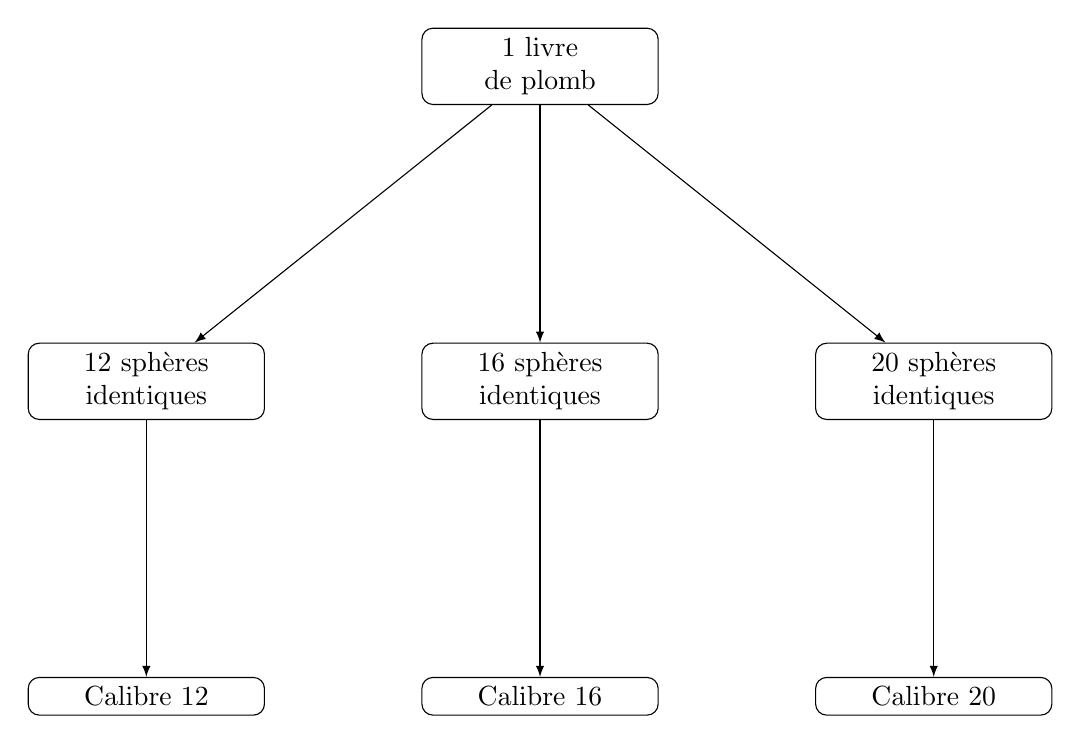
\begin{tikzpicture}[
every node/.style={
draw,
rounded corners,
align=center,
minimum width=3cm
}
]

\node (L) at (0,0)
{1 livre\\de plomb};

\node (C12) at (-5,-4)
{12 sphères\\identiques};

\node (C16) at (0,-4)
{16 sphères\\identiques};

\node (C20) at (5,-4)
{20 sphères\\identiques};

\node (K12) at (-5,-8)
{Calibre 12};

\node (K16) at (0,-8)
{Calibre 16};

\node (K20) at (5,-8)
{Calibre 20};

\draw[-latex] (L) -- (C12);
\draw[-latex] (L) -- (C16);
\draw[-latex] (L) -- (C20);

\draw[-latex] (C12) -- (K12);
\draw[-latex] (C16) -- (K16);
\draw[-latex] (C20) -- (K20);

\end{tikzpicture}

\caption{Principe historique de définition des calibres de chasse.}
\label{fig:origine_calibres}

\end{figure}

\end{comment}

\begin{figure}[htbp]
\centering

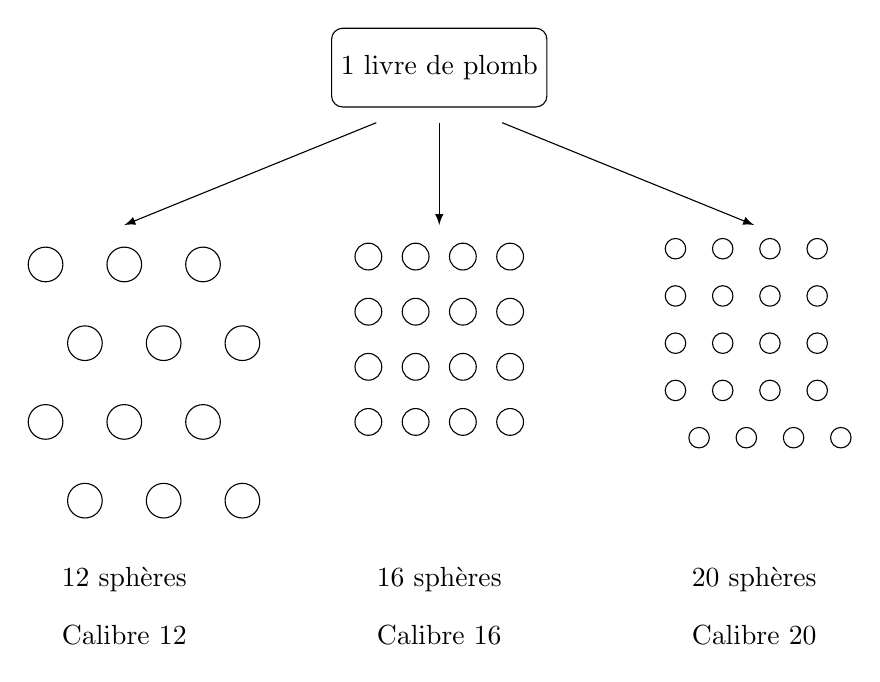
\begin{tikzpicture}[scale=1]

% Livre de plomb
\node[draw,rounded corners,
minimum width=2.5cm,
minimum height=1cm]
(L)
at (0,0)
{1 livre de plomb};

% Flèches
\draw[-latex] (-0.8,-0.7) -- (-4,-2);
\draw[-latex] (0,-0.7) -- (0,-2);
\draw[-latex] (0.8,-0.7) -- (4,-2);

% Calibre 12
\foreach \x/\y in {
-5.0/-2.5,-4.0/-2.5,-3.0/-2.5,
-4.5/-3.5,-3.5/-3.5,-2.5/-3.5,
-5.0/-4.5,-4.0/-4.5,-3.0/-4.5,
-4.5/-5.5,-3.5/-5.5,-2.5/-5.5}
{
\draw (\x,\y) circle (0.22);
}

\node at (-4,-6.5)
{12 sphères};

\node at (-4,-7.2)
{Calibre 12};

% Calibre 16
\foreach \x/\y in {
-0.9/-2.4,-0.3/-2.4,0.3/-2.4,0.9/-2.4,
-0.9/-3.1,-0.3/-3.1,0.3/-3.1,0.9/-3.1,
-0.9/-3.8,-0.3/-3.8,0.3/-3.8,0.9/-3.8,
-0.9/-4.5,-0.3/-4.5,0.3/-4.5,0.9/-4.5}
{
\draw (\x,\y) circle (0.17);
}

\node at (0,-6.5)
{16 sphères};

\node at (0,-7.2)
{Calibre 16};

% Calibre 20
\foreach \x/\y in {
3.0/-2.3,3.6/-2.3,4.2/-2.3,4.8/-2.3,
3.0/-2.9,3.6/-2.9,4.2/-2.9,4.8/-2.9,
3.0/-3.5,3.6/-3.5,4.2/-3.5,4.8/-3.5,
3.0/-4.1,3.6/-4.1,4.2/-4.1,4.8/-4.1,
3.3/-4.7,3.9/-4.7,4.5/-4.7,5.1/-4.7}
{
\draw (\x,\y) circle (0.13);
}

\node at (4,-6.5)
{20 sphères};

\node at (4,-7.2)
{Calibre 20};

\end{tikzpicture}

\caption{Origine historique des calibres de chasse : plus le nombre de sphères obtenues à partir d'une livre de plomb est élevé, plus leur diamètre est faible.}
\label{fig:origine_historique_calibres}

\end{figure}

\section{Conséquence du système}

Plus le nombre associé au calibre est élevé :

\begin{itemize}
    \item plus les sphères sont petites ;
    \item plus le diamètre du canon est faible.
\end{itemize}

Cette relation est donc inverse de l'intuition habituelle.

\begin{figure}[htbp]
\centering

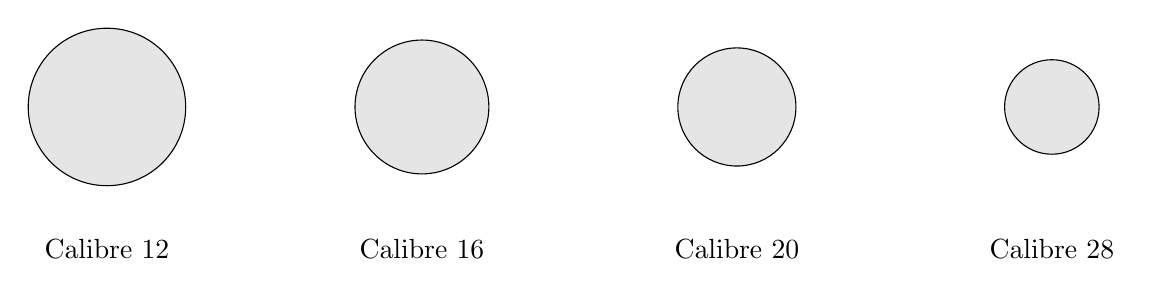
\begin{tikzpicture}

\draw[fill=gray!20] (0,0) circle (1.0);
\node at (0,-1.8) {Calibre 12};

\draw[fill=gray!20] (4,0) circle (0.85);
\node at (4,-1.8) {Calibre 16};

\draw[fill=gray!20] (8,0) circle (0.75);
\node at (8,-1.8) {Calibre 20};

\draw[fill=gray!20] (12,0) circle (0.60);
\node at (12,-1.8) {Calibre 28};

\end{tikzpicture}

\caption{Lorsque le numéro du calibre augmente, le diamètre diminue.}
\label{fig:diametres_calibres}

\end{figure}

\section{Le calibre 12}

Le calibre 12 est aujourd'hui le plus répandu.

Il offre un excellent compromis entre :

\begin{itemize}
    \item masse de charge ;
    \item portée pratique ;
    \item polyvalence.
\end{itemize}

\section{Le calibre 16}

Le calibre 16 fut longtemps très populaire.

Son utilisation a diminué avec la généralisation du calibre 12.

Il reste néanmoins apprécié par certains chasseurs.

\section{Le calibre 20}

Le calibre 20 est souvent choisi pour :

\begin{itemize}
    \item la réduction du poids de l'arme ;
    \item le confort de transport ;
    \item certaines formes de chasse active.
\end{itemize}

\section{Le calibre 28}

Le calibre 28 est moins répandu.

Il est principalement utilisé dans des applications spécialisées.

\section{Le calibre .410}

Le calibre .410 constitue une exception importante.

Contrairement aux autres calibres de chasse, sa désignation correspond
approximativement au diamètre du canon exprimé en pouces.

\begin{figure}[htbp]
\centering

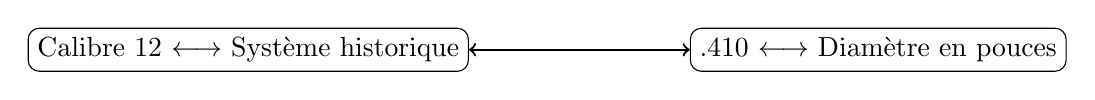
\begin{tikzpicture}

\node[draw,rounded corners]
(H)
at (-4,0)
{Calibre 12 $\longleftrightarrow$ Système historique};

\node[draw,rounded corners]
(D)
at (4,0)
{.410 $\longleftrightarrow$ Diamètre en pouces};

\draw[<->,thick]
(H)
--
(D);

\end{tikzpicture}

\caption{Le .410 constitue une exception au système traditionnel des calibres de chasse.}
\label{fig:cas_410}

\end{figure}

\section{Comparaison des diamètres}

Les différents calibres présentent des diamètres internes différents.

Cependant, ces différences restent relativement modestes.

\begin{figure}[htbp]
\centering

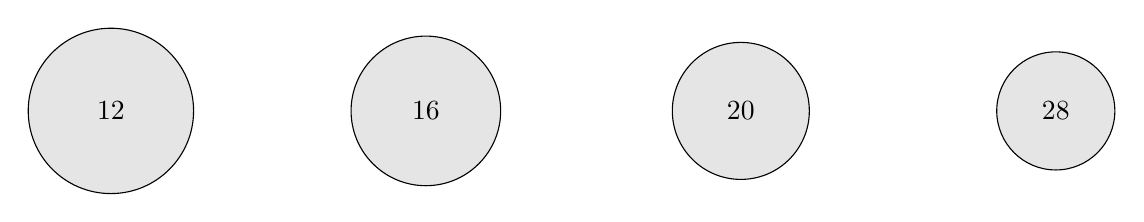
\begin{tikzpicture}

\draw[fill=gray!20] (0,0) circle (1.05);
\node at (0,0) {12};

\draw[fill=gray!20] (4,0) circle (0.95);
\node at (4,0) {16};

\draw[fill=gray!20] (8,0) circle (0.87);
\node at (8,0) {20};

\draw[fill=gray!20] (12,0) circle (0.75);
\node at (12,0) {28};

\end{tikzpicture}

\caption{Comparaison qualitative des diamètres internes des principaux calibres de chasse.}
\label{fig:comparaison_calibres}

\end{figure}

\section{Influence sur la charge}

Le calibre influence directement :

\begin{itemize}
    \item la quantité de grenaille ;
    \item la masse de poudre ;
    \item les performances possibles.
\end{itemize}

\section{Longueur de chambre}

Le calibre ne doit pas être confondu avec la longueur de chambre.

Par exemple :

\begin{itemize}
    \item 12/65 ;
    \item 12/70 ;
    \item 12/76 ;
    \item 12/89.
\end{itemize}

Ces désignations correspondent à des cartouches de même calibre mais de
longueurs différentes.

\begin{figure}[htbp]
\centering

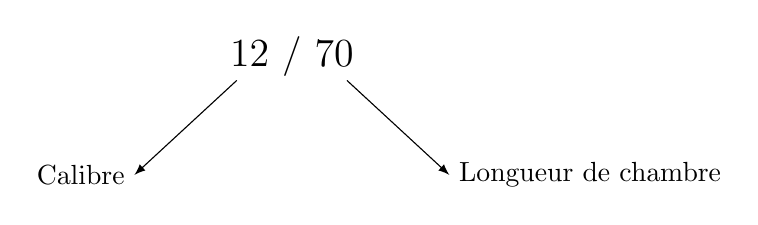
\begin{tikzpicture}

\node[font=\Large] (T) at (0,0)
{12 / 70};

\draw[-latex]
(-0.7,-0.3)
--
(-2,-1.5);

\node[left]
at (-2,-1.5)
{Calibre};

\draw[-latex]
(0.7,-0.3)
--
(2,-1.5);

\node[right]
at (2,-1.5)
{Longueur de chambre};

\end{tikzpicture}

\caption{Exemple de lecture d'une désignation de cartouche de chasse.}
\label{fig:designation_1270}

\end{figure}

\section{Polyvalence du calibre 12}

Le succès du calibre 12 s'explique notamment par sa très grande polyvalence.

Il permet l'utilisation d'une large variété de chargements.

\section{Choix du calibre}

Le choix dépend notamment :

\begin{itemize}
    \item du type de chasse ;
    \item du poids souhaité pour l'arme ;
    \item des munitions disponibles ;
    \item des préférences du tireur.
\end{itemize}

\section{Idées reçues}

Un calibre plus important n'implique pas nécessairement une efficacité
supérieure.

Les performances dépendent également :

\begin{itemize}
    \item du chargement ;
    \item du projectile ;
    \item de la distance ;
    \item du tireur.
\end{itemize}

\section{Vers les chargements}

Le calibre constitue l'un des paramètres essentiels d'une cartouche de chasse.

Le chapitre suivant examinera plus en détail les différents chargements de
grenaille.

\section{À retenir}

\begin{aretenir}

\begin{itemize}
    \item Les calibres de chasse reposent sur une convention historique.
    \item Plus le numéro est élevé, plus le diamètre est faible.
    \item Le calibre 12 est aujourd'hui le plus répandu.
    \item Le calibre .410 constitue une exception.
    \item Le calibre ne doit pas être confondu avec la longueur de chambre.
\end{itemize}

\end{aretenir}
